\begin{frame}
\frametitle{QFPL}
\begin{block}{http://qfpl.io/}

\includegraphics[height=0.24\textheight]{image/qfpl-io.png}
\end{block}
\end{frame}

\begin{frame}
\frametitle{FP}
\begin{center}
Quick disclaimer
\end{center}
\end{frame}

\begin{frame}
\frametitle{FP}
\begin{center}
YOW! is not a Functional Programming conference, but
\end{center}
\end{frame}

\begin{frame}
\frametitle{FP}
\begin{center}
Functional Programming has won the programming debate
\end{center}
\end{frame}

\begin{frame}
\frametitle{FP}
\begin{center}
nearly 20 years ago, and by \emph{more than a teensy bit}
\end{center}
\end{frame}

\begin{frame}
\frametitle{FP}
\begin{center}
FP is strictly superior
\end{center}
\end{frame}

\begin{frame}
\frametitle{FP}
\begin{center}
Second place is so distant that the only ethical response is swift dismissal
\end{center}
\end{frame}

\begin{frame}
\frametitle{FP}
\begin{center}
and you might not believe me
\end{center}
\end{frame}

\begin{frame}
\frametitle{FP}
\begin{center}
and that's OK
\end{center}
\end{frame}

\begin{frame}
\frametitle{FP}
\begin{center}
I will wait


\includegraphics[height=0.1\textheight]{image/man-looking-at-watch.jpg}
\end{center}
\end{frame}

\begin{frame}
\frametitle{FP}
\begin{center}
or maybe I have it all wrong
\end{center}
\end{frame}

\begin{frame}
\frametitle{FP}
\begin{center}
but the point is, some parts of this talk will simply assume it
\end{center}
\end{frame}

\begin{frame}
\frametitle{FP}
\begin{center}
Hope that's cool with you!
\end{center}
\end{frame}

\begin{frame}
\begin{center}
Why aviation?
\end{center}
\end{frame}

\begin{frame}
\frametitle{Aviation}
\begin{block}{My house is near this airport}
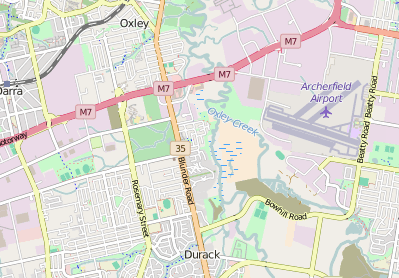
\includegraphics[height=0.5\textheight]{image/archerfield-map.png}
\end{block}
\end{frame}

\begin{frame}
\frametitle{Aviation}
\begin{block}{and I'd see this on my way home}
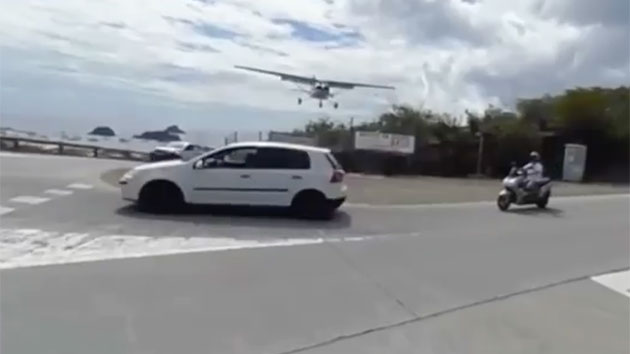
\includegraphics[height=0.5\textheight]{image/aeroplane-approach.jpg}
\end{block}
\end{frame}

\begin{frame}
\frametitle{Aviation}
\begin{block}{This is me on my way home}
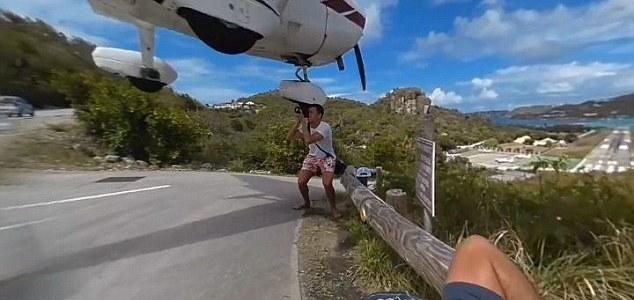
\includegraphics[height=0.5\textheight]{image/aeroplane-graze-photographer.jpg}
\end{block}
\end{frame}

\begin{frame}
\frametitle{Aviation}
\begin{block}{In November 2015, I did this}

\includegraphics[height=0.5\textheight]{image/flight-school-google.png}
\end{block}
\end{frame}

\begin{frame}
\frametitle{A domestic argument ensued}
\begin{block}{My lovely wife Amanda was like}

\includegraphics[height=0.5\textheight]{image/thought-bubble-dollars.png}
\end{block}
\end{frame}

\begin{frame}
\frametitle{A compromise was reached}
\begin{block}{and I was like}

\includegraphics[height=0.3\textheight]{image/tom-cruise.png}
\end{block}
\end{frame}

\begin{frame}
\frametitle{The argument was over}
\begin{block}{and Amanda was like}

\includegraphics[height=0.5\textheight]{image/thought-bubble-good-point.png}
\end{block}
\end{frame}

\begin{frame}
\frametitle{Pilot Licences}
\begin{block}{There are (loosely) four levels of pilot licence}
\begin{enumerate}
\item RPL
  \begin{itemize}
  \item \tiny{MTOW <= 1500kg}
  \item \tiny{no navigation beyond 25nm (46km) from departure point}
  \item \tiny{day time, VFR only}
  \item \tiny{class 1 or 2 aviation medical for >1 PAX}
  \end{itemize}
\item PPL
  \begin{itemize}
  \item \tiny{MTOW <= 5700kg}
  \item \tiny{can navigate}
  \item \tiny{no commercial ops}
  \item \tiny{class 1 or 2 aviation medical for >1 PAX}
  \end{itemize}
\item CPL
  \begin{itemize}
  \item \tiny{commercial ops}
  \item \tiny{class 1 aviation medical}
  \end{itemize}
\item ATPL
  \begin{itemize}
  \item \tiny{>= 1500 hours for aeroplane category}
  \item \tiny{>= 1000 hours for helicopter category}
  \end{itemize}
\end{enumerate}
\end{block}
\end{frame}
